\section*{25/09/2023}
\section{Concetti fondamentali e di ripasso}
\subsection{Elementi di fisica II}
Tratteremo il problma del trasporto ed accumulo di elettroni nei semiconduttori.\\
Il trasporto è legato al campo elettromagnetico mentre la teoria dell'acucumulo è legata all'effetto che si verifica nei condensatori.\\
Gli elettroni si muovono per legge di Coulomb e Lorentz.
La Legge di Lorentz non si usa più (perchè?).

Per Coulomb:
%
\begin{equation*}
    F = q \cdot \mathcal{E} = q\cdot \nabla\phi 
\end{equation*}
%
\begin{equation*}
    F = -\nabla U
\end{equation*}
%
Dove U[Joule] è l'energia potenziale.
si perviene allora alla legge:
%
\begin{equation*}
    U = -q \Phi
\end{equation*}
%
dove $\Phi$[V] è il potenziale elettrico.

Si preferisce usare la grandezza elettronVolt [eV] dove:
$1 eV = 1.6 \cdot 10^{-19} J$

Gli elementi che ci interessano fanno parte del gruppo IV della tabella periodica, insieme alla III ed alla V
%
\begin{figure}[hbt!]
    \centering
    \begin{tabular}{ccc}
        III  & IV   & V\\
        $B$  & $C$  & $P$\\
        $Al$ & $^{14}Si$ & As \\
        $Ge$ & $^{32}Ge$ & Sb\\
        $Jn$ &  & \\
    \end{tabular}
    \caption{Caption}
    \label{fig:enter-label}
\end{figure}
%
B e P sono usati per drogaggio ed ..

Come si struttura il cristallo semiconduttore:
figura..\\ \\
%
\subsection{Elementi di meccanica quantistica}
Una base di fisica quantistica è necessaria perchè mi permetterà di affrontare i semiconduttori ed i dispositivi elettronici sfruttando leggi matematiche classiche (Fisica I) ma con opportune osservazioni dedotte dalla meccanica quantistica, trattazione valida nel caso di particelle (o corpi) a bassa energia.\\
Ho introdotto la sezione facendo riferimento relazioni ''quantistiche'' e ''classiche'', ora devo spiegare che differenza c'è tra i due:
%
\paragraph{Meccanica classica}
Detta in maniera semplice, le leggi della meccanica classica descrivono il mondo
macroscopico (visibile) ma non quelli microscopici, dove la grandezza dei corpi è
confrontabile con quella di atomi e molecole.

Più in dettaglio, la meccanica classica descrive il moto di un corpo attraverso la posizione $\underline{r}$ nello spazio e la sua quantità di moto $\underline{p} = m \cdot \underline{v}$ per istanti di tempo $t > 0$. Tramite le formule classiche, siamo ingrado di ricavare l'energia totale $E$ del corpo data la somma dell'energia cinetica e potenziale.
inoltre, energia e quantità di moto sono grandezze continue e cioè possono assumere qualsiasi valore!\\
%
\paragraph{Meccanica quantistica}
La meccanica quantistica si basa su alcuni principi fondamentali:
%
\begin{enumerate}
\item È possibile descrivere una particella in moto per mezzo di un’onda (detta funzione d’onda $\underline{\psi}$) la cui frequenza e lunghezza d’onda sono associate all’energia e quantità di moto, rispettivamente.\\
Queste funzioni d’onda sono la soluzione di una equazione dinamica (l’equazione di Schròdinger) e il loro modulo quadrato è proporzionale alla probabilità di trovare la
particella in un certo stato (posizione, istante, energia, quantità di moto). 

\item Non è possibile conoscere la traiettoria di una particella in senso classico:
energia, quantità di moto, posizione nello spazio-tempo sono note a meno di
una incertezza o indeterminazione che non può essere mai resa nulla. 

\item Nel comportamento collettivo le particelle quantistiche differiscono dalle particelle classiche in quanto la probabilità di trovare due particelle indistinguibili (ad esempio due elettroni) insieme in un dato stato non è pari al prodotto delle probabilità di trovare in quello stato ciascuna delle particelle, come nel caso classico, ma è o nulla (particelle di Fermi) o maggiore del prodotto delle probabilità (particelle di Bose). Per le particelle di Fermi vale cioè il principio di esclusione: non vi possono essere due particelle nello stesso stato.

\item Dualmente.al comportamento ondulatorio delle particelle, le onde elettromagnetiche presentano un comportamento corpuscolare, ossia sono associate a pseudoparticelle prive di massa dette fotoni

\end{enumerate}

\begin{exbox}[COS'è SCHRODINGER?]
    Prima di tutto, cos'è stato stazionario?\\
    uno stato stazionario è una situazione in cui le proprietà della particella (come la probabilità di trovarsi in una certa posizione o con una certa energia) non cambiano nel tempo. In altre parole, la particella sembra "ferma" o "stazionaria" dal punto di vista delle sue caratteristiche misurabili.

    Immagino di avere un sistema fisico, come ad esempio un elettrone in un atomo.\\
    L'equazione di Schrödinger degli stati stazionari è un modo matematico per descrivere il comportamento di queste particelle.

    Quando risolviamo questa equazione, otteniamo delle soluzioni che corrispondono a diversi livelli di energia consentiti per la particella. In alcuni casi, come quando l'elettrone è confinato in uno spazio specifico, otteniamo un insieme discreto di valori di energia, chiamato spettro discreto.
    
    In casi diversi dallo stato stazionario, come quando l'elettrone può muoversi liberamente in uno spazio, abbiamo un insieme continuo di valori di energia, chiamato spettro continuo.

Infine, ci sono situazioni, come nei solidi cristallini, in cui esistono intervalli specifici di energie in cui le particelle possono trovarsi (bande di energia permessa) e intervalli in cui non possono trovarsi (bande di energia proibita). In questo caso, parliamo di spettro a bande.

In sostanza, l'equazione di Schrödinger ci aiuta a capire come le energie di una particella possono essere distribuite in diverse situazioni fisiche.
\end{exbox}
%
\cleardoublepage
\subsection{Elementi di chimica}
%
\subsubsection{Atomi polielettronici}
Gli atomi polielettronici contengono più di un elettrone.\\
Anche per gli atomi polielettronici è possibile scrivere equazioni d'onda corrette ma non è possibile trovare le soluzioni esatte, si possono solo riportare delle funzioni d'onda approssimate.\\
La difficoltà nel trattare gli atomi polielettronici stà nel fatto che ci sono tanti elettroni attorno al nucleo con la conseguenza che il generico atomo , oltre a subire l'attrazione del nucleo, subisce la repulsione da parte degli altri elettroni.
Ogni elettrone ha funzioni d'onda diverse da quelle degli altri atomi.\\
Tramite evidenze sperimentali, si è osservato che l'elettrone ha una proprietà magnetica intrinseca dovuta alla rotazione dell'elettrone intorno al proprio asse
\begin{psbox}[da reddit]
    Prima di tutto, l'elettrone non sta effettivamente ruotando. Un elettrone non è una piccola sfera. "Spin" è un nome molto sfortunato perché non ha un analogo fisico a cui i non fisici possano aggrapparsi. Pensa se fosse come una carica...gli elettroni hanno una carica. In realtà non ha una causa, fa parte di ciò che *è*  un elettrone. Gli elettroni hanno anche altre proprietà, come la massa. Ogni elettrone ha la stessa massa, ogni elettrone ha la stessa carica.
    Anche gli elettroni hanno un momento angolare... è qui che la cosa diventa strana perché, nel mondo macroscopico, associamo il momento angolare alle cose che ruotano. \\
    A livello quantistico, però, gli elettroni *hanno* semplicemente momento angolare, proprio come hanno massa e carica. Lo chiamiamo "spin", in relazione all'equivalente macroscopico a cui siamo abituati.
\end{psbox}
%
Se prendiamo un atomo polielettronico, tutti gli elettroni dell'atomo ruotano intorno ad assi paralleli; può essere diverso solo il senso della rotazione.
\begin{center}
    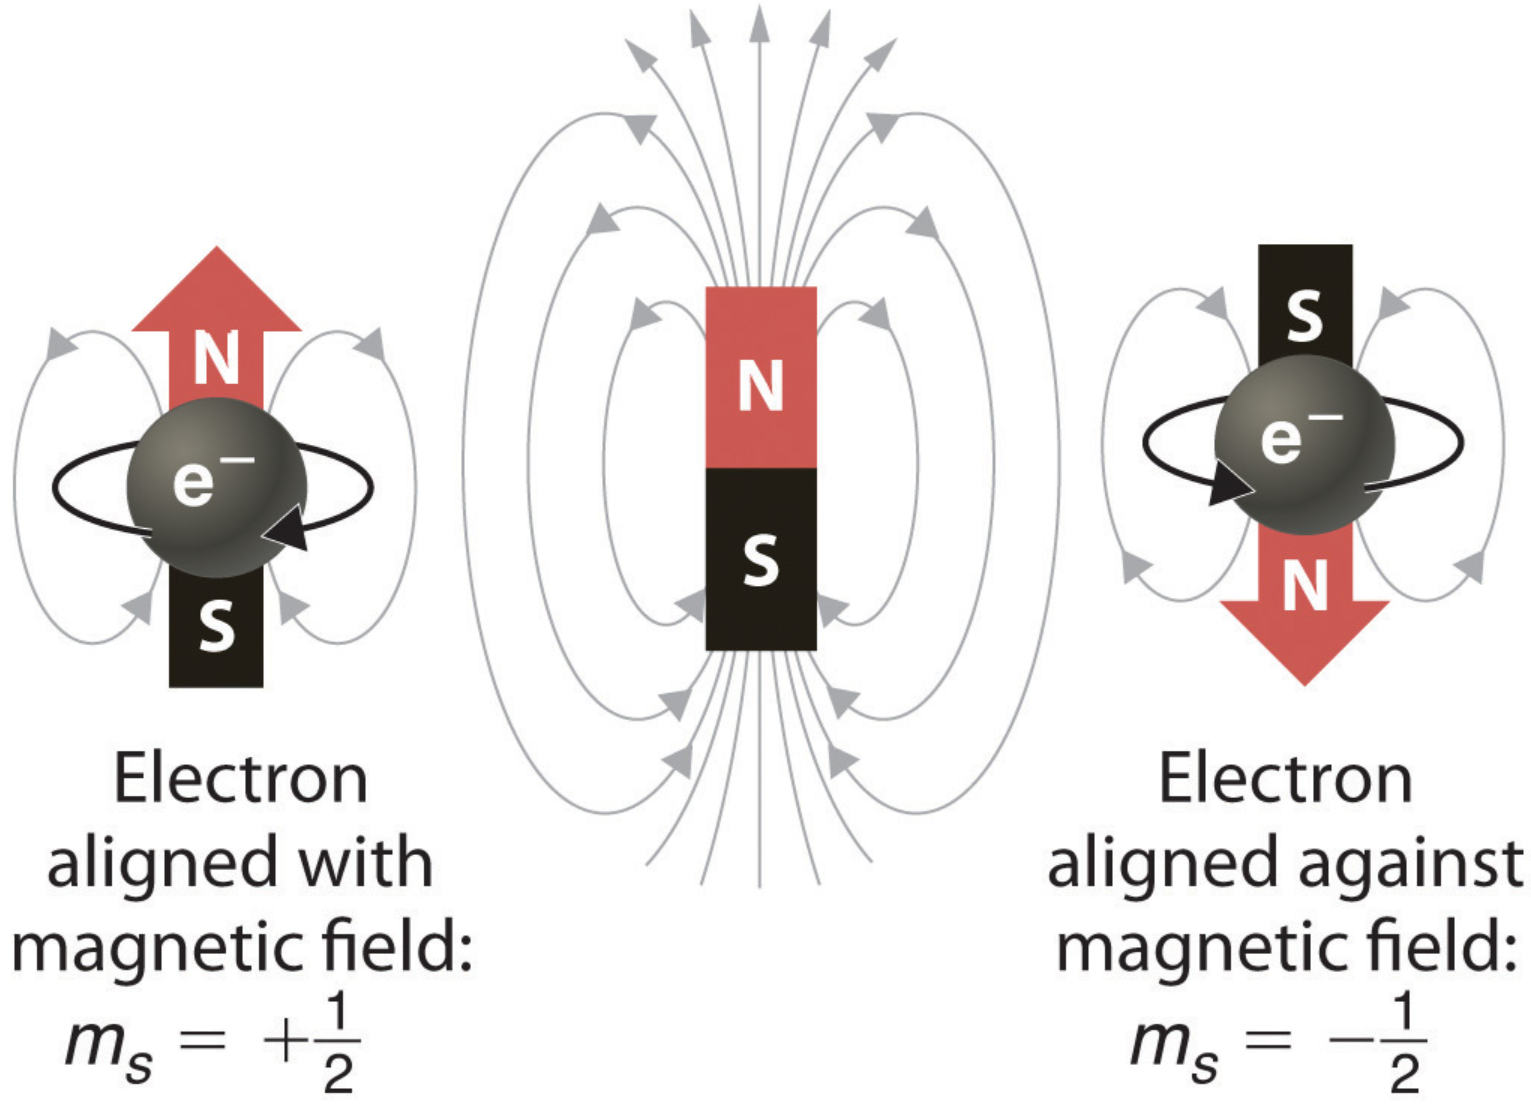
\includegraphics[width=0.5\textwidth]{Immagini_Micro&Nano/Imm_1_Ripasso/spin.png}
    \captionof{figure}{Lo spin di due elettroni in un livello orbitale deve essere opposto}
\end{center}
Questo significa che anche lo spin dell'elettrone è quantizzato ed è necessario introdurre un quarto numero quantico, il numero quantico di spin, che può assumere solo valore di $+\dfrac{1}{2}$ e $-\dfrac{1}{2}$
%
\subsubsection{Riempimento elettronico degli orbitali}
Sò che un atomo è composto da un nucleo circondato da uno o più elettroni, quello che voglio sapere ora è come gli elettroni si dispongono attorno. 
Per il riempimento degli atomi polielettronici vale il principio di esclusione di Pauli: in un atomo non possono esistere due elettroni aventi i quattro numeri quantici uguali. \\
Siccome un orbitale è caratterizzato da tre dei quattro numeri quantici, n, l, m, allora un orbitale può ospitare al massimo due elettroni che si differenziano per il numero quantico di spin, cioè che hanno spin antiparallelo.
%
\begin{exbox}

    %\captionof{figure}{Configurazione degli orbitali}
\begin{center}
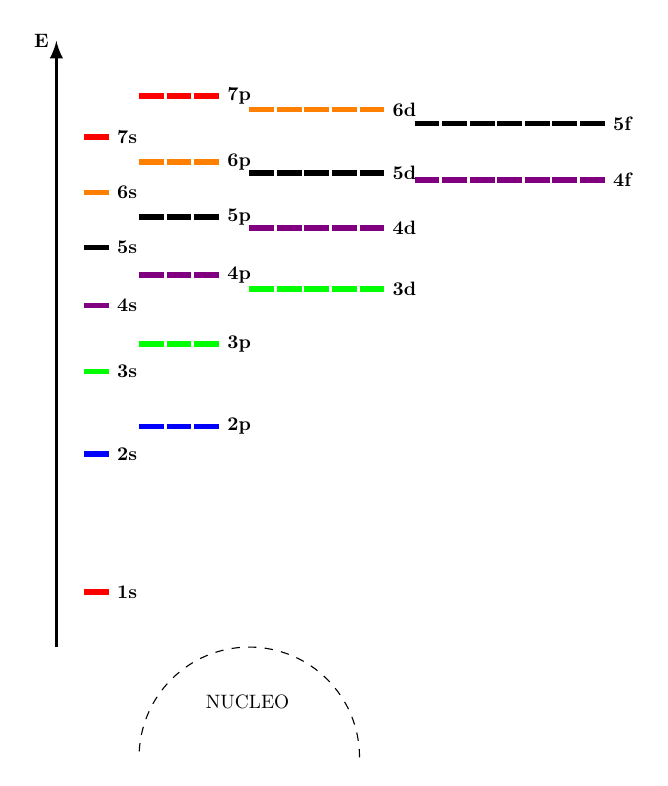
\begin{tikzpicture}[scale=0.7, transform shape]
    %disegno nucleo
    \draw[black, dashed] (5.5,-1) arc (0:180:2);
    \node at (4.35,0)[left]{NUCLEO};
    %disegno y
    \draw[-latex,very thick](0,1)--(0,12)node[left,black]{\textbf{E}};
    %disegno livello 1s
    \draw[line width=2pt,red](0.5,2)--++(0.45,0)node[right,black]{\textbf{1s}};
    %%%%%%%%%%%%%%%%%%%%%%%%%%%%%%%%%%%%%%%%%%%%%%%%%%%%%%%%%%%%%%%%%%%%%%%%%%
    %disegno livello 2s
    \draw[line width=2pt,blue](0.5,4.5)--++(0.45,0)node[right,black]{\textbf{2s}}
    %disegno livello 2p
    (1.5,5)--++(0.45,0) (2,5)--++(0.45,0) (2.5,5)--++(0.45,0)node[right,black]{\textbf{2p}};
    %%%%%%%%%%%%%%%%%%%%%%%%%%%%%%%%%%%%%%%%%%%%%%%%%%%%%%%%%%%%%%%%%%%%%%%%%%
    %disegno livello 3s
    \draw[line width=2pt,green](0.5,6)--++(0.45,0)node[right,black]{\textbf{3s}}
    %disegno livello 3p
    (1.5,6.5)--++(0.45,0) (2,6.5)--++(0.45,0) (2.5,6.5)--++(0.45,0)node[right,black]{\textbf{3p}}
    %disegno livello 3d
    (3.5,7.5)--++(0.45,0) (4,7.5)--++(0.45,0) (4.5,7.5)--++(0.45,0) (5,7.5)--++(0.45,0) (5.5,7.5)--++(0.45,0)node[right,black]{\textbf{3d}};
    %%%%%%%%%%%%%%%%%%%%%%%%%%%%%%%%%%%%%%%%%%%%%%%%%%%%%%%%%%%%%%%%%%%%%%%%%%
    %disegno livello 4s
    \draw[line width=2pt,violet](0.5,7.2)--++(0.45,0)node[right,black]{\textbf{4s}}
    %disegno livello 4p
    (1.5,7.75)--++(0.45,0) (2,7.75)--++(0.45,0) (2.5,7.75)--++(0.45,0)node[right,black]{\textbf{4p}}
    %disegno livello 4d
    (3.5,8.6)--++(0.45,0) (4,8.6)--++(0.45,0) (4.5,8.6)--++(0.45,0) (5,8.6)--++(0.45,0) (5.5,8.6)--++(0.45,0)node[right,black]{\textbf{4d}}
    %disegno livello 4f
    (6.5,9.47)--++(0.45,0) (7,9.47)--++(0.45,0) (7.5,9.47)--++(0.45,0) (8,9.47)--++(0.45,0) (8.5,9.47)--++(0.45,0) (9,9.47)--++(0.45,0) (9.5,9.47)--++(0.45,0)node[right,black]{\textbf{4f}};
    %%%%%%%%%%%%%%%%%%%%%%%%%%%%%%%%%%%%%%%%%%%%%%%%%%%%%%%%%%%%%%%%%%%%%%%%%%
    %disegno livello 5s
    \draw[line width=2pt,black](0.5,8.25)--++(0.45,0)node[right,black]{\textbf{5s}}
    %disegno livello 5p
    (1.5,8.8)--++(0.45,0) (2,8.8)--++(0.45,0) (2.5,8.8)--++(0.45,0)node[right,black]{\textbf{5p}}
    %disegno livello 5d
    (3.5,9.6)--++(0.45,0) (4,9.6)--++(0.45,0) (4.5,9.6)--++(0.45,0) (5,9.6)--++(0.45,0) (5.5,9.6)--++(0.45,0)node[right,black]{\textbf{5d}}
    %disegno livello 5f
    (6.5,10.5)--++(0.45,0) (7,10.5)--++(0.45,0) (7.5,10.5)--++(0.45,0) (8,10.5)--++(0.45,0) (8.5,10.5)--++(0.45,0) (9,10.5)--++(0.45,0) (9.5,10.5)--++(0.45,0)node[right,black]{\textbf{5f}};
    %%%%%%%%%%%%%%%%%%%%%%%%%%%%%%%%%%%%%%%%%%%%%%%%%%%%%%%%%%%%%%%%%%%%%%%%%%
     %disegno livello 6s
    \draw[line width=2pt,orange](0.5,9.25)--++(0.45,0)node[right,black]{\textbf{6s}}
    %disegno livello 6p
    (1.5,9.8)--++(0.45,0) (2,9.8)--++(0.45,0) (2.5,9.8)--++(0.45,0)node[right,black]{\textbf{6p}}
    %disegno livello 6d
    (3.5,10.75)--++(0.45,0) (4,10.75)--++(0.45,0) (4.5,10.75)--++(0.45,0) (5,10.75)--++(0.45,0) (5.5,10.75)--++(0.45,0)node[right,black]{\textbf{6d}};
    %%%%%%%%%%%%%%%%%%%%%%%%%%%%%%%%%%%%%%%%%%%%%%%%%%%%%%%%%%%%%%%%%%%%%%%%%%
     %disegno livello 7s
    \draw[line width=2pt,red](0.5,10.25)--++(0.45,0)node[right,black]{\textbf{7s}}
    %disegno livello 7p
    (1.5,11)--++(0.45,0) (2,11)--++(0.45,0) (2.5,11)--++(0.45,0)node[right,black]{\textbf{7p}};
    %\draw [arrows = {-Stealth[harpoon]}];
\end{tikzpicture}
\captionof{figure}{Configurazione degli orbitali}
\end{center}
   
%
    Consideriamo atmoni neutri non eccitati (detti allo stato fondamentale in cui elettroni non hanno energia sufficiente a fare salti) e sistemiamo gli elettroni seguendo lo schema di energie ed applicando il principio di Paoli.\\
    ES.1:\\
    L'idrogeno è un elemento con numero atomico Z=1. allora si ha un elettrone nell'orbitale 1s.\\
    ES.1:\\
    L'elio è un elemento con numero atomico Z=2. allora l'orbitale 1s sarà pieno.

    Facendo un passo in avanti, considero la regola di Hund: quando ci sono a disposizione più orbitali vuoti della stessa energia, gli elettroni vanno a occupare singolarmente questi orbitali con gli elettroni che anno a ruotare con spin parallelo.\\
    ES.3:\\
    Il carbonio (C) è un elemento con numero atomico Z=6. allora si ha due elettroni in due diversi orbitali 2p con spin parallelo.\\
    da mettere una figura con spin
\end{exbox}
%
\cleardoublepage